\documentclass[11pt,letterpaper]{article}
\usepackage[lmargin=1in,rmargin=1in,tmargin=1in,bmargin=1in]{geometry}
\usepackage{../style/homework}
\usepackage{../style/commands}
\setbool{quotetype}{false} % True: Side; False: Under
\setbool{hideans}{true} % Student: True; Instructor: False

% -------------------
% Content
% -------------------
\begin{document}

\homework{5: Due 06/01}{Science, my lad, is made up of mistakes, but they are mistakes which it is useful to make, because they lead little by little to the truth.}{Jules Verne}

% Problem 1
\problem{10} Define what makes a function linear. What `form' does every linear function of one-variable have?



\newpage



% Problem 2
\problem{10} Being as accurate as possible, sketch the graph of the line $-3x + 5y= 10$.
	\[
	\fbox{
	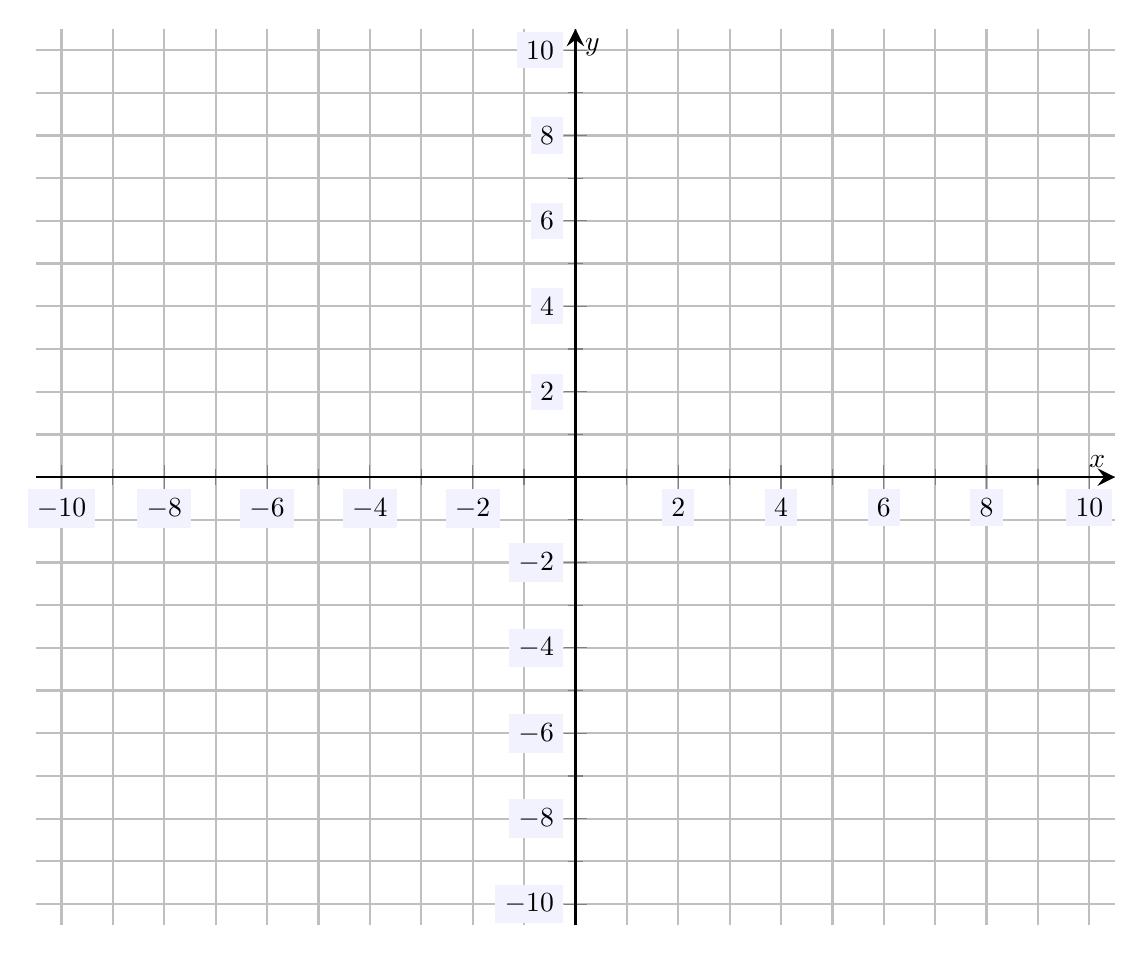
\begin{tikzpicture}[scale=2,every node/.style={scale=0.5}]
	\begin{axis}[
	grid=both,
	axis lines=middle,
	ticklabel style={fill=blue!5!white},
	xmin= -10.5, xmax=10.5,
	ymin= -10.5, ymax=10.5,
	xtick={-10,-8,-6,-4,-2,0,2,4,6,8,10},
	ytick={-10,-8,-6,-4,-2,0,2,4,6,8,10},
	minor tick = {-10,-9,...,10},
	xlabel=\(x\),ylabel=\(y\),
	]
	\end{axis}
	\end{tikzpicture}
	}
	\] 



\newpage



% Problem 3
\problem{10} Determine if the following function is linear. Explain why or why not.
	\begin{table}[!ht]
	\centering
	\begin{tabular}{c|c}
	$x$ & $f(x)$ \\ \hline
	$0.5$ & $26.45$ \\
	$1.8$ & $21.64$ \\
	$3.9$ & $13.87$ \\
	$4.2$ & $13.44$ \\
	$5.5$ & $7.95$ \\
	$8.1$ & $-1.67$
	\end{tabular}
	\end{table}



\newpage



% Problem 4
\problem{10} Consider the linear equation $15x + 3y= 39$. 
        \begin{enumerate}[(a)]
        \item Solve the linear equation for $y$. 
        \item Determine the slope and $y$-intercept for the corresponding line.
        \item Interpret the slope in at least two different ways. 
        \end{enumerate}



\newpage



% Problem 5
\problem{10} Consider the line given by $y= \frac{11}{4}\,x - 6$.
        \begin{enumerate}[(a)]
        \item Put the line in standard form.
        \item Is the point $(-12, -27)$ on the line? Explain.
        \item Is the point $(8, 16)$ on the line? Explain. 
        \end{enumerate} 



\newpage



% Problem 6
\problem{10} A linear function has a table whose values are given below. Find the equation of the linear function. Be sure to specify the slope and $y$-intercept.
	\begin{table}[!ht]
	\centering
	\begin{tabular}{c|c}
	$x$ & $f(x)$ \\ \hline
	$3$ & $5.7$ \\ 
	$4$ & $2.4$ \\
	$7$ & $-7.5$ \\
	$11$ & $-20.7$
	\end{tabular}
	\end{table}



\newpage



% Problem 7
\problem{10} Consider the linear function $f(x)= \dfrac{4 - 3x}{2}$.
	\begin{enumerate}[(a)]
	\item Find the slope of this linear function. 
	\item Interpret the slope two different ways.
	\item Is the linear function increasing, decreasing, or constant? Explain. 
	\item Determine the $y$-intercept for $f(x)$.
	\item Determine the $x$-intercept for $f(x)$.
	\end{enumerate} 



\newpage



% Problem 8
\problem{10} You are driving back to college after summer break. It is 12~pm and you are traveling on the highway at a constant speed of 65~mph. Currently, you are 211~mi from college. Let $D(t)$ denote your distance, in miles, that you are from the college $t$ hours from now. 
	\begin{enumerate}[(a)]
	\item Explain why $D(t)$ is linear.
	\item Find $D(t)$. 
	\item What do the slope and $y$-intercept of $W(t)$ represent in context?
	\item Determine when you will arrive at the college. 
	\end{enumerate} 



\newpage



% Problem 9
\problem{10} Showing all your work, find the equation of the line with slope $-\frac{1}{3}$ that passes through the point $(9, 4)$. 



\newpage



% Problem 10
\problem{10} Showing all your work, find the equation of the line that has $x$-intercept $(-2, 0)$ and $y$-intercept $(0, -5)$. 


\end{document}